\newpage

\section{Appendix}



\subsection{Implementation Details}\label{appendix:hyper}
The hyper parameters used for K-RagRec and their corresponding values are shown in Table~\ref{tab:hyper}. The first part provides the general training setting for K-RagRec. The second part presents the details of ($\text{GNN}^{\text{Indexing}}$, $\text{GNN}^{\text{Encoding}}$). Then we list the Lora and acceleration settings. Lastly, we provide the hyper parameters for retrieval, including candidate item number $M$, popularity selective retrieval policy threshold $p$, retrieve knowledge sub-graphs numbers $K$, and re-ranking knowledge sub-graphs numbers $N$. If not specified, we run all methods three times with different random seeds and report the averaged results.


\begin{table}[htbp]
 \vskip -0.02in
  \centering
  \caption{Basic statistics of three datasets and the KG. "Items in KG" indicates the number of items that appeared in both the KG and the dataset. 
  }
   \vskip -0.1in
    \scalebox{0.6}
{
  \begin{adjustbox}{}
    \begin{tabular}{c|c|c|c}
    \toprule
    \toprule
    \multirow{1}{*}{Datasets} & {MovieLens-1M} & {MovieLens-20M} & {Amazon Book} \\
    \midrule
User  & 6,038 & 138,287 & 6,106,019 \\
Item & 3,533 & 20,720 & 1,891,460 \\
Interaction & 575,281 & 9,995,410 & 13,886,788 \\
Items in KG & 3,498 & 20,139 & 91,700 \\
\midrule
Entitys & 250,631 & 1,278,544 & 186,954\\
Relations &  264   & 436    & 16 \\
KG triples & 348,979 & 1,827,361 & 259,861  \\
    \bottomrule
    \bottomrule
    \end{tabular}%
    \end{adjustbox}
}
 \vskip -0.1in
  \label{tab:datasets}%
\end{table}%

\subsection{Graph Neural Networks}\label{appendix:gnn}
GNNs are a critical technique in graph machine learning and are widely employed in various graph tasks. 
By iteratively updating node representations through aggregating information from neighboring nodes, GNNs effectively capture the underlying topology and relational structure of graphs.
Formally, a typical GNN operation can be formulated as follows:
\begin{equation}
\mathbf{x}_j^{(l+1)}=\mathbf{x}_j^{(l)} \oplus \mathrm{AGG}^{(l+1)}\left(\left\{\mathbf{x}_i^{(l)} \mid i \in \mathcal{N}_{x_j}\right\}\right),
\end{equation}
where $\mathbf{x}_j^{(l+1)}$ express node $j$'s feature on the $l$-th layer, and $\mathcal{N}(x_j)$ is the set of neighbours of node $j$. $\mathrm{AGG}$ is a aggregation function to aggregates
neighbors’ features, and $\oplus$ combines neighbors' information with the node itself.



\begin{table}[htbp]
  % \vskip -0.05in
  \centering
  \caption{Statistics of Hyper Parameters.}
  % \vskip -0.05in
    \scalebox{0.8}
{
  % \begin{adjustbox}{}
    \begin{tabular}{c|c}
    \toprule
    \toprule
    \multirow{1}{*}{Item}  & \multirow{1}{*}{Value}  \\
    \midrule
    batch size & 5  \\
    epochs  & 3  \\
    grad steps & 2 \\
    learning rate & 1e-5 \\
    \midrule
    Indexing layer numbers & 4  \\
    Indexing hidden dimension & 1024  \\
    Encoding layer numbers & 4  \\
    Encoding hidden dimension & 1024  \\
    Encoding head numbers & 4  \\
    \midrule
    lora\_r & 8 \\
    lora\_alpha & 16 \\
    lora\_dropout & 0.1 \\
    int8 & True \\
    fp16 & True \\
    \midrule
    candidate item numbers & 20\\
    threshold $p$ & 50\% \\
    top-$K$ & 3 \\
    top-$N$ & 5 \\
    \bottomrule
    \bottomrule
    \end{tabular}%
    %\end{adjustbox}
}
  \label{tab:hyper}%
  % \vskip -0.06in
\end{table}%



\subsection{More Related Work}\label{appendix:related_work}
The remarkable breakthroughs in LLMs have led to their widespread adoption across various fields, particularly in the recommendations. 
Given powerful reasoning and generalization capabilities, many studies have actively attempted to harness the power of the LLM to enhance recommender systems~\citep{geng2022recommendation,bao2023tallrec,qu2024tokenrec,wei2024llmrec,zhang2023collm}. For example, P5~\citep{geng2022recommendation} proposes an LLM-based recommendation model by unifying pre-training, prompting, and prediction for various recommendation tasks, such as sequential recommendation and rating predictions. Furthermore, Tallrec~\citep{bao2023tallrec} fine-tunes LLM (i.e., LLaMA-7B) to align with recommendation data for sequential recommendations.
To further capture higher-order collaborative knowledge and enhance the model's ability to generalize users and items, TokenRec~\citep{qu2024tokenrec} proposes a masked vector-quantized tokenizer to tokenize users and items in LLM-based recommendations.
Despite their effectiveness, these models often face challenges, such as hallucinations and the lack of up-to-date knowledge.
While fine-tuning can partially mitigate these issues, it is resource-costly and time-consuming due to the massive parameters of LLMs.
To overcome these challenges, we propose a knowledge retrieval augmented recommendation framework that leverages external KGs to provide reliable and up-to-date knowledge instead of costly fine-tuning.


\subsection{Comparison with Existing Methods}
Existing LLM-based recommender systems usually require frequent fine-tuning on specific datasets to address the lack of knowledge and hallucinations, which is time-consuming and costly. To solve these challenges and avoid costly fine-tuning, our work is the first to augment the recommendation performance of LLMs by retrieving structured data (i.e., knowledge graph). Specifically, our approach differs from existing work in the following ways:
\vspace{-0.1in}
 \begin{itemize} [leftmargin=*] 
\setlength{\itemsep}{0pt}
\setlength{\parsep}{0pt}
\setlength{\parskip}{0pt}
\item K-RagRec introduces an indexing GNN to efficiently retrieve structured data to enhance the recommendation capability of LLMs. Although some GraphRAG approaches also introduce GNNs to capture higher-order neighbourhood information, they only apply the last layer of the GNN representation, leading to coarse retrieval~\citep{he2024g, mavromatis2024gnn}. In contrast, our approach leverages the representation of each GNN layer to retrieve nuanced knowledge of both coarse and fine-grained graph structures from KG, achieving a more comprehensive and precise retrieval.
\item In the recommendation domain that pursues inference speed, excessive retrieval time can seriously degrade the user experience resulting in user churn. Although many studies have explored selective retrieval for RAGs~\citep{yan2024corrective,jiang2023active}, it is still an open question to determine whether an item needs to be retrieved and to reduce the retrieval time in the recommendation domain. We propose to use popularity to decide whether an item needs to be retrieved based on power law distribution, which greatly reduces the retrieval time. Table~\ref{tab:time} shows that K-RagRec achieves inference times close to direct inference while maintaining high recommendation accuracy.
\item Typical RAG methods usually incorporate the retrieved content into the prompt as text~\citep{wu2023retrieve,baek2023knowledge}. However, vanilla RAG methods rely on documents and paragraphs often introduce unnecessary noise and even harmful disturbance, which can negatively impact the accuracy and reliability of recommendations. In addition, the structural relationships between entities are overlooked in typical RAG, resulting in the sub-optimal reasoning capability of LLM-based recommender systems. We propose to incorporate the retrieved knowledge subgraphs (Knowledge-GraphRAG) into the query as a graph prompt, which facilitates LLMs to better understand the retrieved knowledge subgraphs and avoids long contexts.
\end{itemize}

\subsection{Comparison with 10 Candidate Items}\label{appendix:10samples}
In this section, we conduct additional experiments to evaluate the effectiveness of K-RagRec with a candidate item number $M=10$. In this setting, we randomly select nine negative samples with the target item. The results are presented in Table~\ref{tab:10samples}. We exclude the results of some backbone LLM models (e.g., LLama-3 and QWEN2), as similar observations as Table~\ref{tab:results} can be found. Observing the experimental results, we can note that our proposed K-RagRec method consistently outperforms all baseline methods on MovieLens and Amazon Book datasets, further highlighting the effectiveness of our framework.

\begin{table}[t]
  % \vskip -0.05in
  \centering
  \caption{ Performance comparison of different KG RAG-enhanced LLM recommendations with candidate item numbers $M=10$ on the MovieLens and Amazon Book dataset and LLama-2-7b across
two metrics. The best performances are labeled in bold. ACC and R@3 denote Accuracy and Recall@3, respectively. }
  % \vskip -0.05in
    \scalebox{0.65}
{
  % \begin{adjustbox}{}
    \begin{tabular}{c|c|c|c|c}
    \toprule
    \toprule
    \multirow{2}{*}{Methods} & \multicolumn{2}{c|}{MovieLens-1M} & \multicolumn{2}{c}{Amazon Book} \\
    \cmidrule{2-5}
    & \multicolumn{1}{c|}{ACC} & \multicolumn{1}{c|}{R@3} & \multicolumn{1}{c|}{ACC} & \multicolumn{1}{c}{R@3}  \\
    \midrule
    KG-Text &0.185  &- &0.142  &-  \\
    KAPING &0.165  &- & 0.119 &-  \\
    PT w/ KG-Text &0.159  &0.493 &0.123  &0.384  \\
    GraphToken w/ RAG &0.512  &0.753 &0.444  & 0.682 \\
    G-retriever &0.469  &0.721 &0.367  &0.610  \\
    \midrule
 K-RagRec &\textbf{0.568}  &\textbf{0.779} &\textbf{0.606}  &\textbf{0.770}  \\
    \bottomrule
    \bottomrule
    \end{tabular}%
    %\end{adjustbox}
}
  \label{tab:10samples}%
  % \vskip -0.06in
\end{table}%

\subsection{Ablation Study Setting}\label{appendix:Abla}
To assess the impact of each module in K-RagRec, we compare the framework with four ablated variants: K-RagRec (\textit{-Indexing}), K-RagRec (\textit{-Popularity}), K-RagRec (\textit{-Re-ranking}), and K-RagRec (\textit{-Encoding}). (1) K-RagRec (\textit{-Indexing}) eliminates the $\text{GNN}^{\text{Indexing}}$ and stores semantic information of PLM in the knowledge vector database. For the retrieved nodes, we extract their second-order sub-graphs as the retrieved knowledge sub-graphs. (2) K-RagRec (\textit{-Popularity}) does not apply the popularity selective retrieval policy and retrieves all items from the user's historical interactions. (3) (\textit{-Re-ranking}) removes the re-ranking module and inputs the knowledge sub-graphs directly. (4) K-RagRec (\textit{-Encoding}) removes the $\text{GNN}^{\text{Encoding}}$ and replaces it with a trainable soft prompt. The retrieved knowledge sub-graphs will be added to the prompt as triples (e.g., \textit{\{Moonraker, film writer film, Christopher Wood (writer)\}}).


\subsection{\textbf{Generalization Study}}\label{appendix:General}
To evaluate the generalization capability of our proposed framework in the zero-shot setting, we trained a version of the model on the MovieLens-1M dataset and assessed it on the MovieLens-20M and Amazon Book datasets. The experiment results are shown in Table~\ref{tab:transferability}. 
We note that although the K-RagRec performance in the zero-shot setting is slightly degraded when compared to the well-trained model in Table~\ref{tab:results},  it still demonstrates 21.6\% improvement over SOTA baselines on the MovieLens-20M dataset. 
Furthermore, despite the differences between the book recommendation and movie recommendation tasks, the model trained on MovieLens-1M delivers about 8.7\% improvement in the zero-shot setting compared to prompt-tuned baselines on the Amazon Book dataset.
The experimental results demonstrate that K-RagRec exhibits strong generalization capabilities and is adaptable across different domains.


\begin{table}[t]
  % \vskip -0.05in
  \centering
  \caption{ The generalization results for our K-RagRec model in a zero-shot setting. In this setting, our models are trained on MovieLens-1M dataset and evaluated on MovieLens-20M and Amazon Book datasets.  ACC and R@$k$ denote Accuracy
and Recall@$k$, respectively.}
  \vskip -0.05in
    \scalebox{0.57}
{
  % \begin{adjustbox}{}
    \begin{tabular}{c|c|c|c|c|c|c|c}
    \toprule
    \toprule
    \multirow{2}{*}{Models}  & \multirow{2}{*}{Methods} & \multicolumn{3}{c|}{MovieLens-20M} & \multicolumn{3}{c}{Amazon Book} \\
    \cmidrule{3-8}
    & & \multicolumn{1}{c|}{ACC} & \multicolumn{1}{c|}{R@3} & \multicolumn{1}{c|}{R@5} & \multicolumn{1}{c|}{ACC} & \multicolumn{1}{c|}{R@3} & \multicolumn{1}{c}{R@5} \\
    \midrule
 \multirow{2}{*}{LLama2} & K-RagRec &0.539  &0.740 &0.795 &0.390  &0.581 &0.671    \\
  & Lora w/K-RagRec &0.539  &0.783 &0.863 &0.405 &0.580 &0.796   \\
  \midrule
\multirow{2}{*}{LLama3} &K-RagRec  &0.597 &0.797 &0.839 &0.428 &0.628 &0.706 \\
 & Lora w/K-RagRec  &0.611  &0.775 &0.814 &0.424 &0.622 &0.732  \\
 \midrule
\multirow{2}{*}{QWEN} &K-RagRec  &0.507 &0.769 &0.861 &0.418 &0.612  &0.687\\
 & Lora w/K-RagRec &0.545  &0.814 &0.897 &0.441 &0.623 &0.706   \\
    \bottomrule
    \bottomrule
    \end{tabular}%
    %\end{adjustbox}
}
  \label{tab:transferability}%
  \vskip -0.06in
\end{table}%

\begin{table}[t]
  % \vskip -0.05in
  \centering
  \caption{Quantitative comparison of hallucination on the MovieLens-1M dataset. $\Delta$ denotes the reduction in hallucinations for K-RagRec compared to Direct Inference.}
  % \vskip -0.05in
    \scalebox{0.75}
{
  % \begin{adjustbox}{}
    \begin{tabular}{c|c|c|c}
    \toprule
    \toprule
    \multirow{1}{*}{Models}
    & \multicolumn{1}{c|}{Direct Inference} & \multicolumn{1}{c|}{K-RagRec} & \multicolumn{1}{c}{$\Delta$}\\
    \midrule
    LLama-2 &39.1\%  &2.7\% &93.1\% \\
    \midrule
 QWEN2 &4.7\% &0.9\% & 80.9\% \\
    \bottomrule
    \bottomrule
    \end{tabular}%
    %\end{adjustbox}
}
  \label{tab:hallucination}%
  % \vskip -0.06in
\end{table}%

\subsection{Study of Hallucination}
In this section, we present a qualitative analysis of hallucinations in the LLama-2-7b and QWEN2 models on the MovieLens dataset. Specifically, we include a few fictional movies in the candidate items to observe the probability of the fictional movie being recommended. We compare direct recommendations and recommendations augmented with K-RagRec, and the results are shown in Table~\ref{tab:hallucination}. We note that K-RagRec significantly reduced hallucinations by 93.1\% compared to direct inference on LLama-2. In contrast to LLama-2, QWEN2 rarely recommends fictional movies. Nevertheless, K-RagRec reduced hallucinations by 80.9\%, demonstrating the effectiveness of our approach in addressing hallucinations.


\begin{table}[t]
  % \vskip -0.05in
  \centering
  \caption{ Performance comparison of different KG RAG-enhanced LLM recommendation methods on the cold-start dataset and QWEN2 across three metrics. The best performances are labeled in bold. ACC and R@$k$ denote Accuracy and Recall@$k$, respectively. }
  % \vskip -0.05in
    \scalebox{0.85}
{
  % \begin{adjustbox}{}
    \begin{tabular}{c|c|c|c}
    \toprule
    \toprule
    \multirow{1}{*}{Methods}
    & \multicolumn{1}{c|}{ACC} & \multicolumn{1}{c|}{R@3} & \multicolumn{1}{c}{R@5} \\
    \midrule
    PT w/ KG-Text &0.106  &0.239 &0.395  \\
    GraphToken w/ RAG &0.258  &0.473 &0.620 \\
    G-retriever &0.185  &0.384 &0.488  \\
    \midrule
 K-RagRec &\textbf{0.406}  &\textbf{0.705} &\textbf{0.834}  \\
    \bottomrule
    \bottomrule
    \end{tabular}%
    %\end{adjustbox}
}
  \label{tab:cold_start}%
  % \vskip -0.06in
\end{table}%

\subsection{Study of Cold Start Recommendation}
The cold start problem is an important issue in most recommendation research. To comprehensively evaluate our approach, we particularly design a case study to evaluate the model's recommendation performance under the cold-start setting. Specifically, we construct a separate cold-start dataset based on the MovieLens dataset that only contains these identified cold-start items as target items. We compare K-RagRec with three KG RAG-enhanced LLM recommendation methods, and the experiment results are shown in Table~\ref{tab:cold_start}. The results demonstrate that our proposed K-RagRec still has satisfactory performance under the cold-start recommendation scenario, highlighting the effectiveness of our framework in all the cases.





\begin{table}[t]
  % \vskip -0.05in
  \centering
  \caption{ 
   Comparison of different GNN Encoders on the MovieLens-1M dataset and LLama-2-7b across three metrics. We use bold fonts to label the best performance. ACC and R@k denote Accuracy and Recall@k, respectively.}
  \vskip -0.05in
    \scalebox{0.75}
{
  % \begin{adjustbox}{}
    \begin{tabular}{c|c|c|c}
    \toprule
    \toprule
    \multirow{1}{*}{GNN Types}  & \multirow{1}{*}{ACC} & \multirow{1}{*}{R@3} &\multirow{1}{*}{R@5}  \\
    \midrule
    GCN~\citep{kipf2016semi} & 0.397 & 0.704 & 0.809 \\
    GAT~\citep{velickovic2017graph}  & 0.420 & 0.693 & 0.804 \\
    Graph Transformer~\citep{shi2020masked} & \textbf{0.429} & \textbf{0.711} &0.779 \\
    GraphSAGE~\citep{hamilton2017inductive} &0.418  &0.699  &\textbf{0.823} \\
    \bottomrule
    \bottomrule
    \end{tabular}%
    %\end{adjustbox}
}
  \label{tab:gnn}%
  \vskip -0.06in
\end{table}%
\subsection{Study of Four GNN Encoders}\label{appendix:gnn encoder}
To further understand the generality of our proposed approach, we conduct a comparative study of four variants applying different GNN encoders. Specifically, we compare GCN~\citep{kipf2016semi}, GAT~\citep{velickovic2017graph}, Graph Transformer~\citep{shi2020masked}, and GraphSAGE~\citep{hamilton2017inductive} as four K-RagRec variants of GNN encoder.
Specifically, Graph Convolutional Network (GCN)~\citep{kipf2016semi} first introduces convolutional operations to graph-structured data. By aggregating features from neighboring nodes, GCN facilitates the learning of rich node representations. GraphSAGE~\citep{hamilton2017inductive} learns an aggregation function that samples and combines features from a node's local neighborhood in an inductive setting, enabling the effective use of new nodes.
Graph Attention Network (GAT)~\citep{velickovic2017graph} further incorporates attention mechanisms, allowing the model to dynamically assign varying attention to neighboring nodes, thereby enhancing the focus on the most relevant information.
Inspired by the success of the transformer, the Graph Transformer~\citep{shi2020masked} adapts transformer architectures to graph data, enhancing the modeling of graphs, particularly textual graphs.

We report the experiment results on the MovieLens-1M dataset and the LLama-2-7b backbone in Table~\ref{tab:gnn}. 
It is noted that the GCN Encoder variant method performs second-best on the Recall@5 metric, although it is slightly worse than other GNN encoders on the Accuracy metric.
Overall, four GNN encoder variants exhibit close performance on the MovieLens dataset, highlighting the generality and robustness of our framework across different GNN encoders.




\begin{table}[t]
  % \vskip -0.05in
  \centering
  \caption{ 
   Comparison of different GNN layers on the Amazon Book dataset and LLama-2-7b across three metrics. ACC and R@k denote Accuracy and Recall@k, respectively.}
  % \vskip -0.05in
    \scalebox{0.75}
{
  % \begin{adjustbox}{}
    \begin{tabular}{c|c|c|c}
    \toprule
    \toprule
    \multirow{1}{*}{GNN Layers}  & \multirow{1}{*}{ACC} & \multirow{1}{*}{R@3} &\multirow{1}{*}{R@5}  \\
    \midrule
    3 layers&  0.496 & 0.653 & 0.736 \\
    4 layers& 0.506 & 0.690 & 0.780 \\
    5 layers& 0.498 &0.656 &0.729 \\
    \bottomrule
    \bottomrule
    \end{tabular}%
    %\end{adjustbox}
}
  \label{tab:gnn_layer}%
  % \vskip -0.06in
\end{table}%
\subsection{Study of GNN Layer Numbers}\label{appendix:gnn layer}
In this subsection, we evaluate the impact of the number of GNN layers on model performance. We vary the numbers of the GNN layer numbers in the range of \{3, 4, 5\} and test on the Amazon Book dataset and LLama-2-7b across three metrics. As observed in Table~\ref{tab:gnn_layer}, the model performance first improves and then decreases as the number of GNN layers increases, and the model achieves the best results across the three metrics when setting the number of GNN layers is set to four. 
Therefore, a smaller number of GNN layers may not have sufficient depth to capture the intricate relationships and dependencies in the graph, leading to sub-optimal performance. On the other hand, too many layers can result in indistinguishable node representations. Thus, selecting the optimal number of GNN layers is crucial for effective model training.


\begin{figure*}[htbp]
% \vskip -0.1in
\centering
\subfigure[Accuracy]{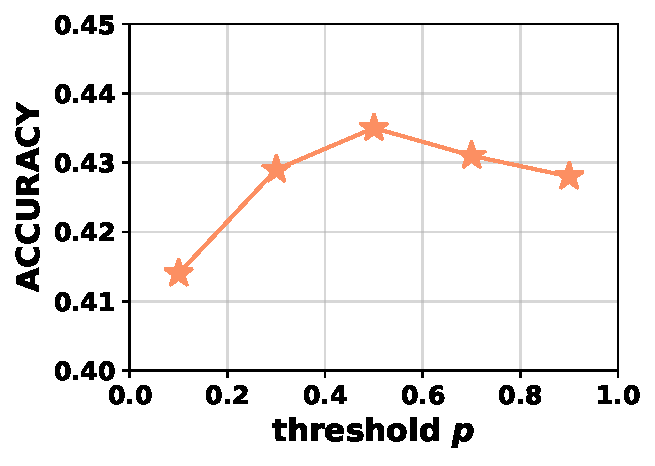
\includegraphics[width=0.65\columnwidth]{figures/parameters/para-acc2.pdf}}
\subfigure[Recall@5]{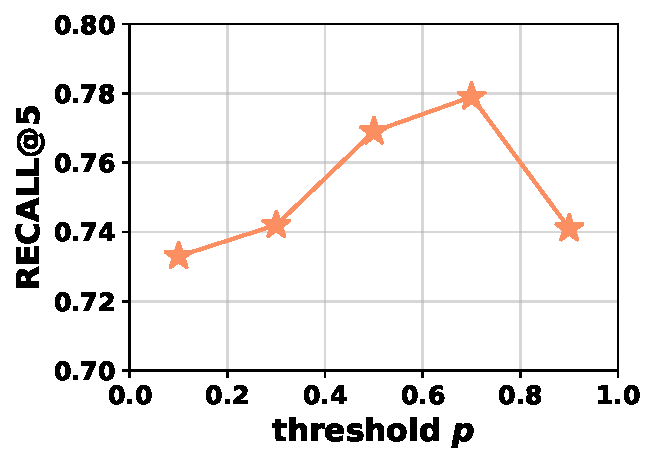
\includegraphics[width=0.65\columnwidth]{figures/parameters/para-recall52.pdf}}
\subfigure[Inference Time]{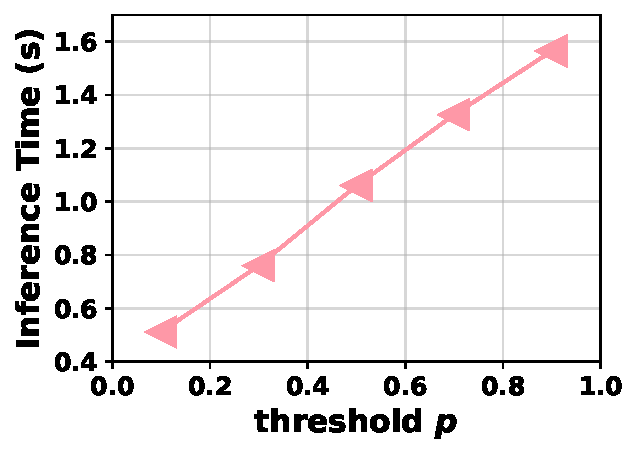
\includegraphics[width=0.65\columnwidth]{figures/parameters/para-time2.pdf}}

\vskip -0.13in
\caption{
Effect of popularity selective retrieval policy threshold $p$ on MovieLens-1M and LLama-2-7b across metrics Accuracy,
Recall@5 and inference time (seconds) for K-RagRec.
}\label{fig:para1}
\vskip -0.23in
\end{figure*}

\begin{figure*}[htbp]
% \vskip -0.4in
\centering
\subfigure[Amazon Book: Accuracy]{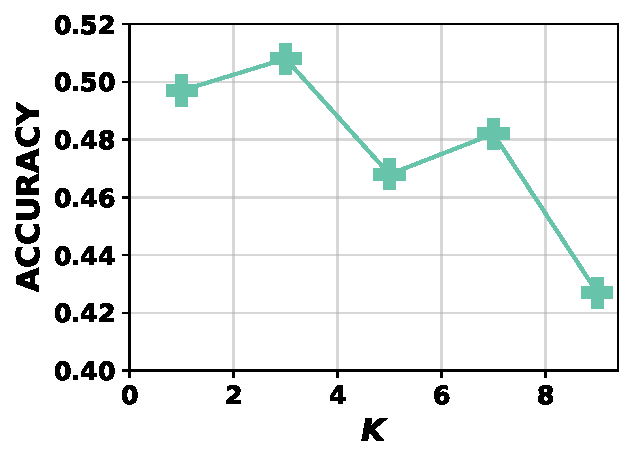
\includegraphics[width=0.65\columnwidth]{figures/parameters/para-k-book-acc.pdf}}
\subfigure[Amazon Book: Recall@3]{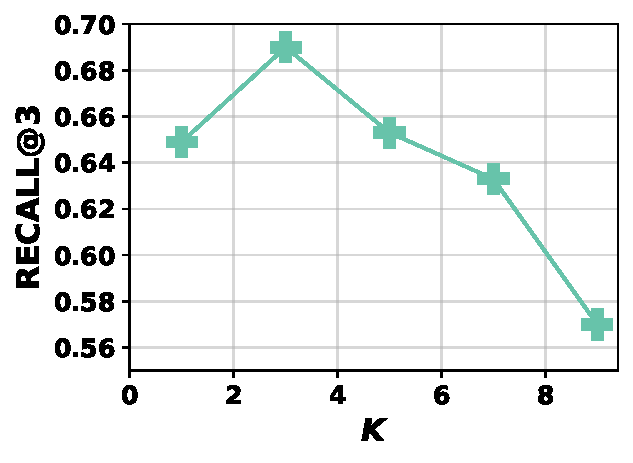
\includegraphics[width=0.65\columnwidth]{figures/parameters/para-k-book-recall3.pdf}}
\subfigure[Amazon Book: Recall@5]{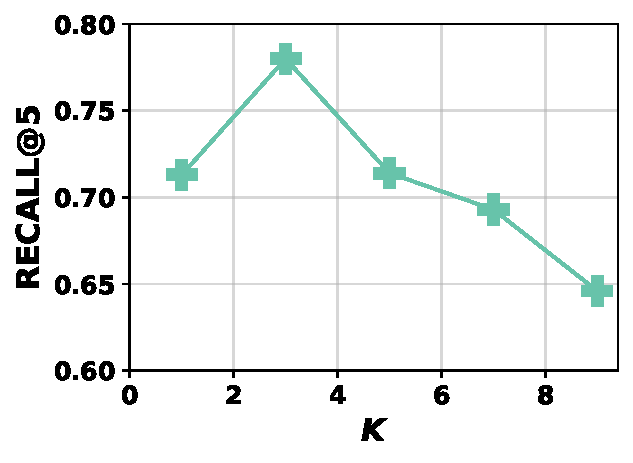
\includegraphics[width=0.65\columnwidth]{figures/parameters/para-k-book-recall5.pdf}}

\vskip -0.13in
\caption{
Effect of retrieved knowledge sub-graph numbers $K$ on Amazon Book datasets and LLama-2-7b across metrics Accuracy,
Recall@3 and Recall@5 for K-RagRec.
}\label{fig:parak}
\vskip -0.23in
\end{figure*}

\begin{figure*}[htbp]
% \vskip -0.4in
\centering
\subfigure[Amazon Book: Accuracy]{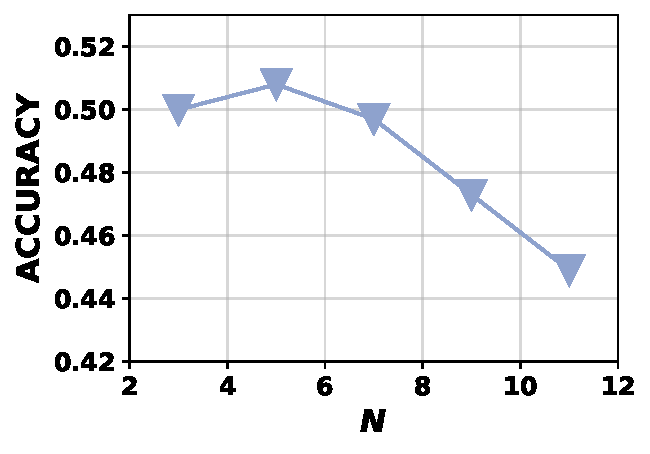
\includegraphics[width=0.65\columnwidth]{figures/parameters/para-reranking-book-acc.pdf}}
\subfigure[Amazon Book: Recall@3]{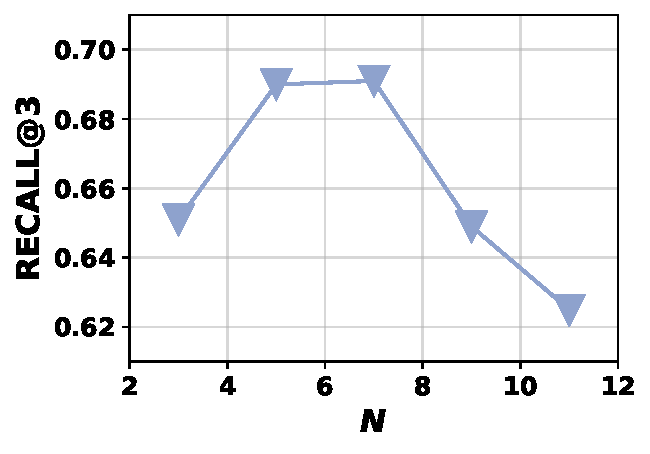
\includegraphics[width=0.65\columnwidth]{figures/parameters/para-reranking-book-recall3.pdf}}
\subfigure[Amazon Book: Recall@5]{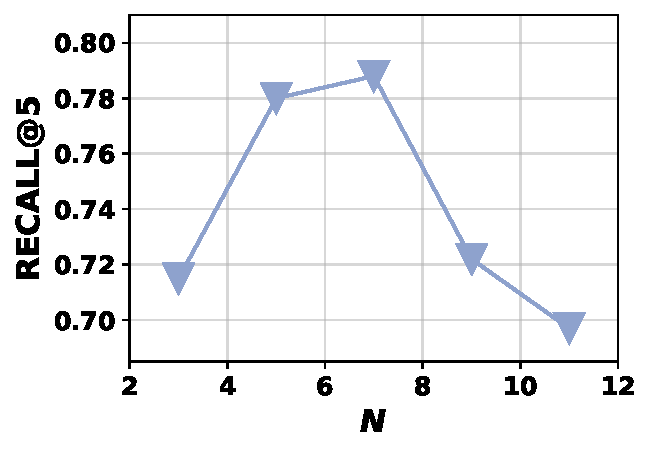
\includegraphics[width=0.65\columnwidth]{figures/parameters/para-reranking-book-recall5.pdf}}

\vskip -0.13in
\caption{
Effect of re-ranking knowledge sub-graph numbers $N$ on Amazon Book datasets and LLama-2-7b across metrics Accuracy,
Recall@3 and Recall@5 for K-RagRec.
}\label{fig:paraK}
\vskip -0.13in
\end{figure*}


\subsection{Used Prompt}\label{appendix:prompt}
In this part, we present the prompts designed for movie recommendations and book recommendations. We show two examples in Table~\ref{tab:prompt}, and set the candidate items $M$ equal to 20. For inference, we leverage the model to make the prediction based on the user's recent watching history and candidate items. 


\begin{table*}[t]
  \centering
  \caption{Example of the used prompt for K-RagRec. The user's recent watching/reading history and candidate items are marked in red and blue, respectively.}
  % \vskip -0.1in
    \scalebox{0.8}{
  \begin{tabularx}{\textwidth}{l|X}
    % \begin{tabular}{p{4.19em}p{73.94em}}
    \toprule
    \multicolumn{1}{c|}{Datasets}  & \multicolumn{1}{c}{Used Prompt} \\
    \midrule
       Movies & Below is an instruction that describes a task, paired with an input that provides further context. Write a response that appropriately completes the request. Instruction: Given the user's watching history, select a film that is most likely to interest the user from the options.  Watching history: \red{\{"History of the World: Part I", "Romancing the Stone", "Fast Times at Ridgemont High", "Good Morning, Vietnam", "Working Girl", "Cocoon", "Splash", "Pretty in Pink", "Terms of Endearment", "Bull Durham"\}}. Options: \blue{\{A: "Whole Nine Yards", B: "Hearts and Minds", C: "League of Their Own", D: "Raising Arizona", E: "Happy Gilmore", F: "Brokedown Palace", G: "Man Who Knew Too Much", H: "Light of Day", I: "Tin Drum", J: "Blair Witch Project", K: "Red Sorghum", L: "Flintstones in Viva Rock Vegas", M: "Anna, N: Roger \& Me" O: "Land and Freedom", P: "In Love and War", Q: "Go West", R: "Kazaam", S: "Thieves", T: "Friends \& Lovers"\}}. Select a movie from options A to T that the user is most likely to be interested in. \\
       \midrule
       Books & Below is an instruction that describes a task, paired with an input that provides further context. Write a response that appropriately completes the request. Instruction: Given the user's reading history, select a book that is most likely to interest the user from the options.  Watching history: \red{\{"Practice Makes Perfect: Spanish Verb Tenses", "NTC's Dictionary of Common Mistakes in Spanish", "Streetwise Spanish Dictionary/Thesaurus", "Buscalo! (Look It Up!) : A Quick Reference Guide to Spanish Grammar and Usage", "La lengua que heredamos: Curso de espaol para bilinges", "Vox Diccionario De Sinonimos Y Antonimos", "Schaum's Outline of Spanish Vocabulary", "Nos Comunicamos (Spanish Edition)", "The Oxford Spanish Business Dictionary", "Bilingual Dictionary of Latin American Spanish"\}}. Options: \blue{\{"A: Folk and Fairy Tales, Childcraft (Volume 3)", B: "The Waves", C: "Dead End Kids: Gang Girls and the Boys They Know", D: "Opera Stars in the Sun: Intimate Glimpes of Metropolitan Opera Personalities", E: "Five-Minute Erotica", F: "Spanish Verbs: Oxford Minireference", G: "Motorcycle Maintenance Techbook: Servicing \& Minor Repairs for All Motorcycles \& Scooters", H: "Father and Son: A Study of Two Temperaments (Classic, 20th-Century, Penguin)", I: "Manga Mania Fantasy Worlds: How to Draw the Amazing Worlds of Japanese Comics", J: "MCSE Designing a Windows Server 2003 Active Directory \& Network Infrastructure: Exam 70-297 Study Guide and DVD Training System", K: "The Atmospheric Boundary Layer (Cambridge Atmospheric and Space Science Series)", L: "St. Augustine and St. Johns County: A pictorial history", M: "A Will to Survive: Indigenous Essays on the Politics of Culture, Language, and Identity", N: "Saved: A Guide to Success With Your Shelter Dog", O: "Mosaic (Star Trek Voyager)", P: "Fantastical Tarot: 78-Card Deck", Q: "American Sign Language-A Look at Its History, Structure and Community", R: "Warrior's Heart (Zebra Historical Romance)", S: "The New Money Management: A Framework for Asset Allocation", T: "Megabrain"\}}. Select a book from options A to T that the user is most likely to be interested in. \\
    \bottomrule
    % \end{tabular}%
    \end{tabularx}%
    }
  \label{tab:prompt}%
\end{table*}%